\subsubsection{Modbus}\label{par:modbus}
\paragraph{Краткое резюме}
Открытый коммуникационный протокол для обмена данными между сетевыми устройствами, основанный на архитектуре ведущий - ведомый (master-slave). Обмен данными представляет собой транзакции, состоящие
из запросов и ответов \cite{__2017-1}. 

\textbf{Достоинства протокола} \cite{__2016}:
\begin{itemize}
	\item открытость;
	\item простота;
	\item массовость;
	\item дешевизна;
	\item отсутствие необходимости в специальных интерфейсных контроллерах \cite{__2010};
	\item надёжный метод контроля ошибок.
\end{itemize}

\textbf{Недостатки протокола}:
\begin{itemize}
	\item невозможность передавать данные по мере получения, необходим постоянный опрос slave - устройств \cite{__2010};
	\item сетевые адреса прописываются на этапе проектирования системы и не могут быть изменены \cite{__2017-1};
	\item длина запроса ограничена, а данные могут быть запрошены только из последовательно расположенных регистров;
	\item не предусмотрен способ, с помощью которого подчиненное устройство могло бы обнаружить потерю связи с ведущим;
	\item соответствие регистров типам измерений и измерительным каналам не регламентировано, что может приводить к несовместимости протоколов
	счетчиков разных типов даже одного производителя;
	\item нет защиты от сторонних несканционированных команд, нельзя передавать конфиденциальные данные \cite{_modbus_2021}.
\end{itemize}

\paragraph{Принцип работы}
\subparagraph{Физический уровень}
Протокол \mb может быть использован со следующими интерфейсами:
\begin{itemize}
	\item \textbf{RS-232/422/485}:  последовательные интерфейсы, широко распространенные в промышленности. Интерфейсы RS-422/485 обеспечивают дальность сигнала до 1200 метров. Используются протоколы \mb RTU/ASCII
	\item \textbf{TCP/IP}: физическим каналом передачи данных могут любые ethernet-ин\-терфейсы. Используется протокол \mb \tcp.
\end{itemize}
Существует 3 разновидности протокола \mb{} \cite{_modbus_2021}:
\begin{enumerate}
	\item \mb{} \textit{ASCII}: в котором данные кодируются символами из таблицы ASCII (рис. 1) и передаются в шестнадцатеричном формате и данный формат протокола встречается довольно редко;
	\item \mb{} \textit{RTU}: самый распространенный вариант протокола \mb, который кодирует данные в двоичном формате и разделяет пакеты с помощью временного интервала;
	\item \mb{} \textit{TCP}:  данные кодируются в двоичном формате и упаковываются в TCP - пакет, для передачи по IP-сетям и предназначен для работы в локальных сетях.
\end{enumerate}

На \refris{fig:modbusphys} показан пример построения схемы контроля за неким объектом при помощи протокола \mb{} \cite{advantech__2019}.

\begin{figure}[p]
	\centering
	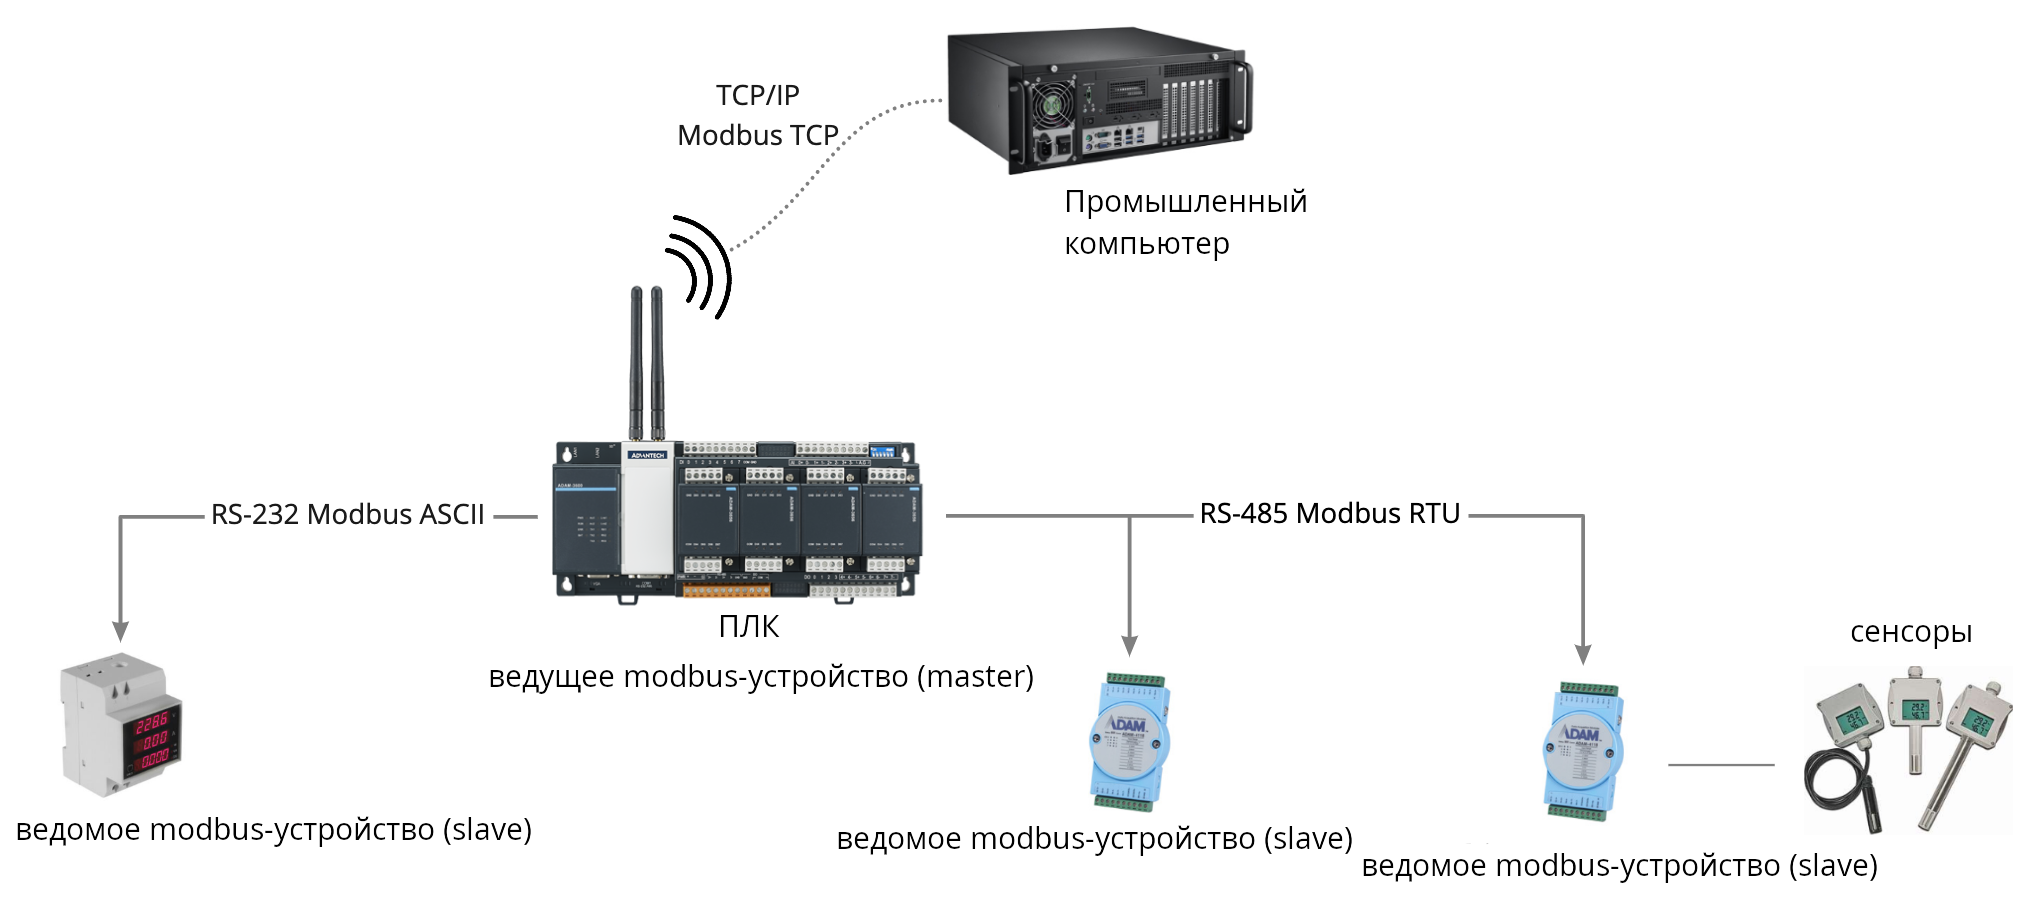
\includegraphics[width=0.9\linewidth]{images/modbus_phys}
	\caption{Физический уровень протокола \mb{}}
	\label{fig:modbusphys}
\end{figure}

\subparagraph{Логический (канальный) уровень}
Протокол \mb предполагает $1$ ведущее устройство и до $247$ ведомых. Обмен данными начинается ведущим устройством. Ведомые не могут начинать передачу и обмениваться данными между собой. В любой момент времени может происходить только один акт обмена. Структуры пакетов \mb при работе 3 способами приведены на \refris{fig:modbusstruct}.
\begin{figure}[p]
	\centering
	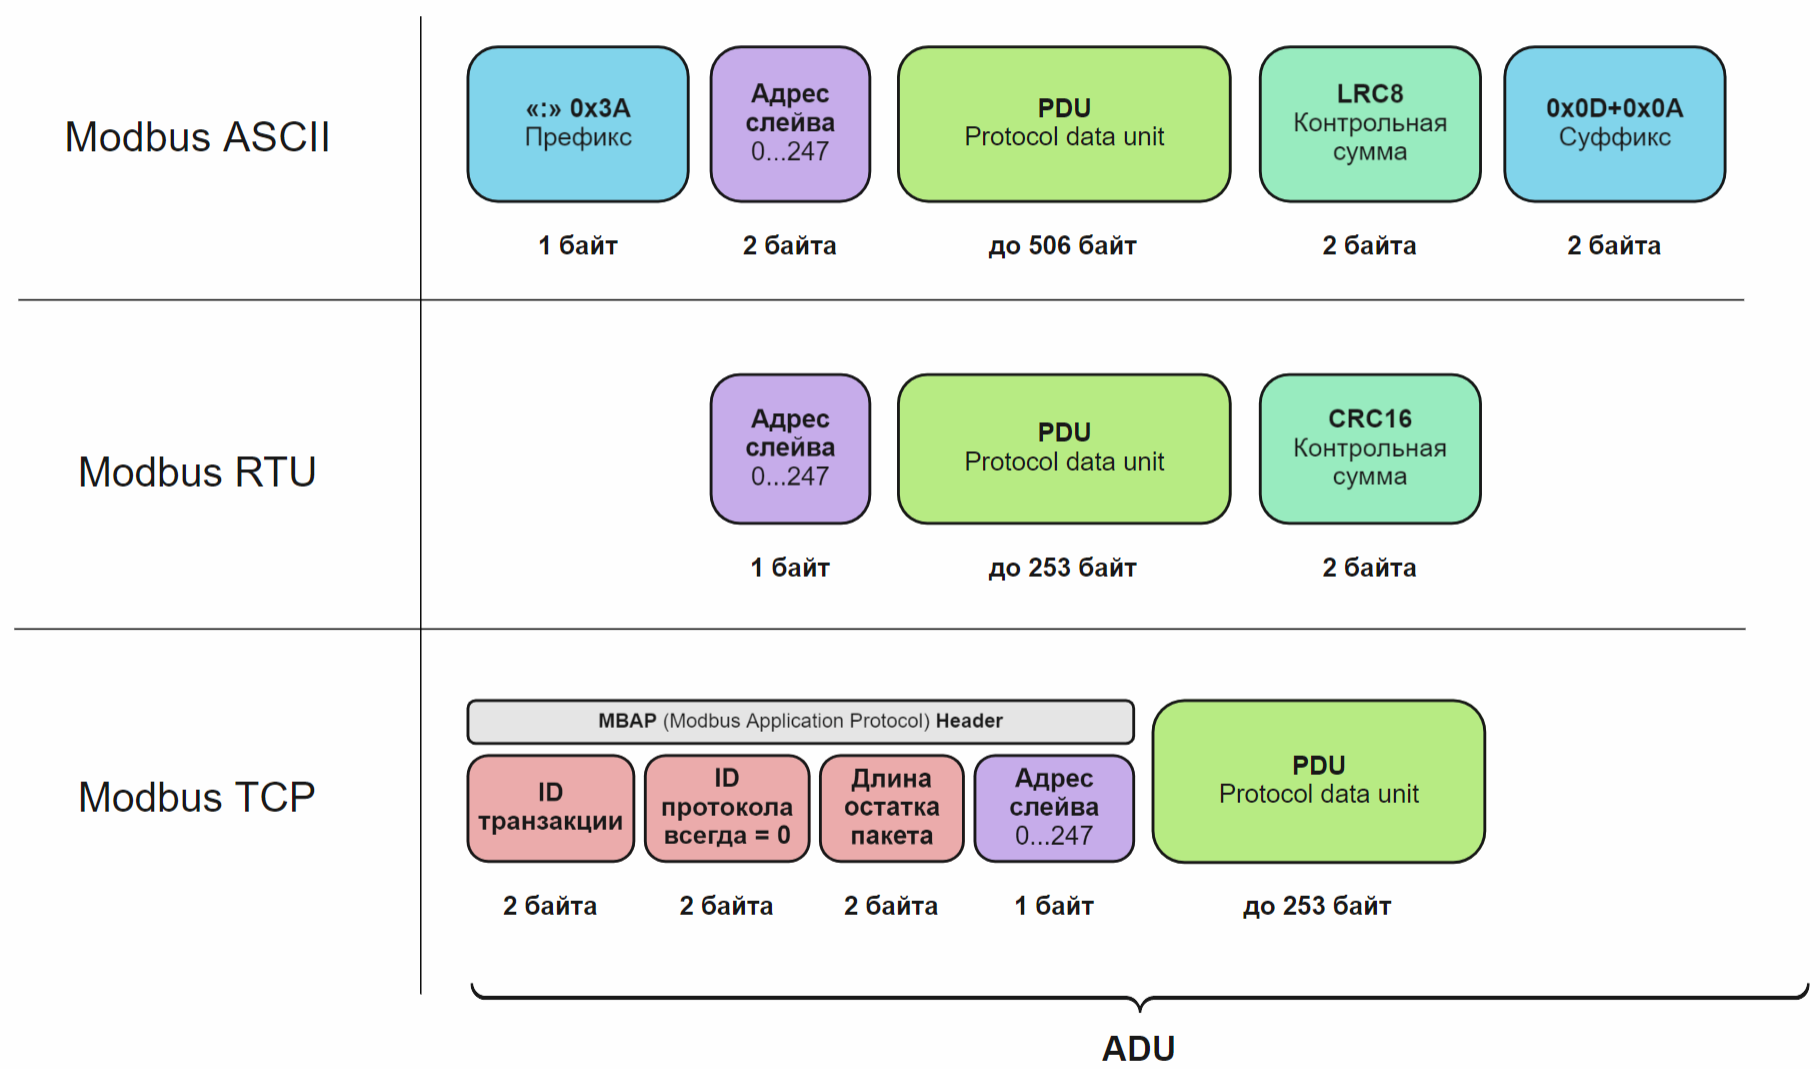
\includegraphics[width=0.9\linewidth]{images/modbus_struct}
	\caption{Структура пакета \mb}
	\label{fig:modbusstruct}
\end{figure}


\subparagraph{Modbus RTU} \label{par:modbusrtu}
Сообщение начинает восприниматься как новое после паузы длиной в $14$ бит. На \refris{fig:modbuspdu} показан формат пакета.
\begin{figure}
	\centering
	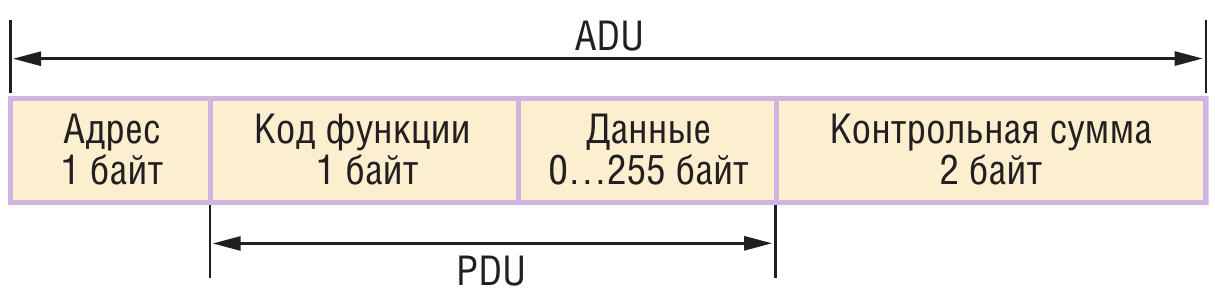
\includegraphics[width=\linewidth]{images/modbus_PDU}
	\caption{Формат кадра протокола \mb \textit{RTU}}
	\label{fig:modbuspdu}
\end{figure}
У пакета есть следующие поля \cite{__2010}:
\begin{itemize}
	\item \textbf{Адрес:} содержит адрес ведомого устройства. Адрес отправляется даже при ответе на запрос мастера, тем самым всегда понятно, откуда пришёл ответ;
	\item \textbf{Код функции:} говорит модулю о том, что ему необходимо сделать;
	\item \textbf{Данные:} тут может содержаться информация о параметрах, которые используются в исполнении команд мастера или показания, передаваемые мастеру;
	\item \textbf{Контрольная сумма:} используется для проверки целостности пакета.
\end{itemize}

\subparagraph{Modbus TCP}
Данный протокол используется для того, чтобы подключить устройства, работающие по протоколу \mb к сети \textit{Internet} \cite{__2018-1}. То есть, в соответствии со стандартом \osi (см. \refris{fig:osi}) на транспортном уровне используется протокол \tcp, а на прикладном -- \mb. В этом случае проверка целостности пакета ложится на протокол \tcp. Структура протокола \mb \tcp приведена на \refris{fig:modbustcp}. 
\begin{figure}
	\centering
	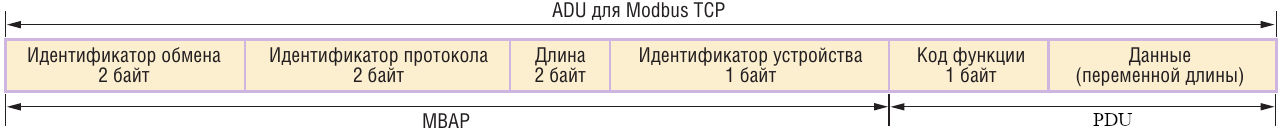
\includegraphics[width=1\linewidth]{images/modbus_TCP}
	\caption{Формат кадра протокола \mb \tcp}
	\label{fig:modbustcp}
\end{figure}
У пакета есть следующие поля \cite{__2010}:
\begin{itemize}
	\item \textbf{Идентификатор обмена:} используется для идентификации сообщения в случае,	когда в пределах одного TCP - соединения клиент посылает серверу несколько сообщений без ожидания ответа после каждого сообщения;
	\item \textbf{Идентификатор протокола:} всегда выставлен на 0 (как и у протокола \tcp);
	\item \textbf{Длина:} указывает количество следующих байтов;
	\item \textbf{Идентификатор устройства:} адрес slave - устройства;
	\item \textbf{Код функции:} аналогично \refpar{par:modbusrtu};
	\item \textbf{Данные:} аналогично \refpar{par:modbusrtu}.
\end{itemize}

Как можно заметить, \mb \textit{RTU} оказывается ``вшит'' в пакет \tcp, тем самым получается \mb \tcp. На \refris{fig:modbustcp_ip} показан принцип работы такой системы \cite{__2010}:
\begin{itemize}
	\item коды функций передаются с прикладного уровня на транспортный (\mb -- \tcp), добавление заголовка \tcp;
	\item передача на сетевой уровень, добавление блока \textit{IP};
	\item передача на канальный уровень, а затем на физический (\textit{Ethernet})
\end{itemize}
После прохождения через канал связи пакет начинает обратное движение согласно модели \osi (см. \refris{fig:osi}). 
\begin{figure}[h]
	\centering
	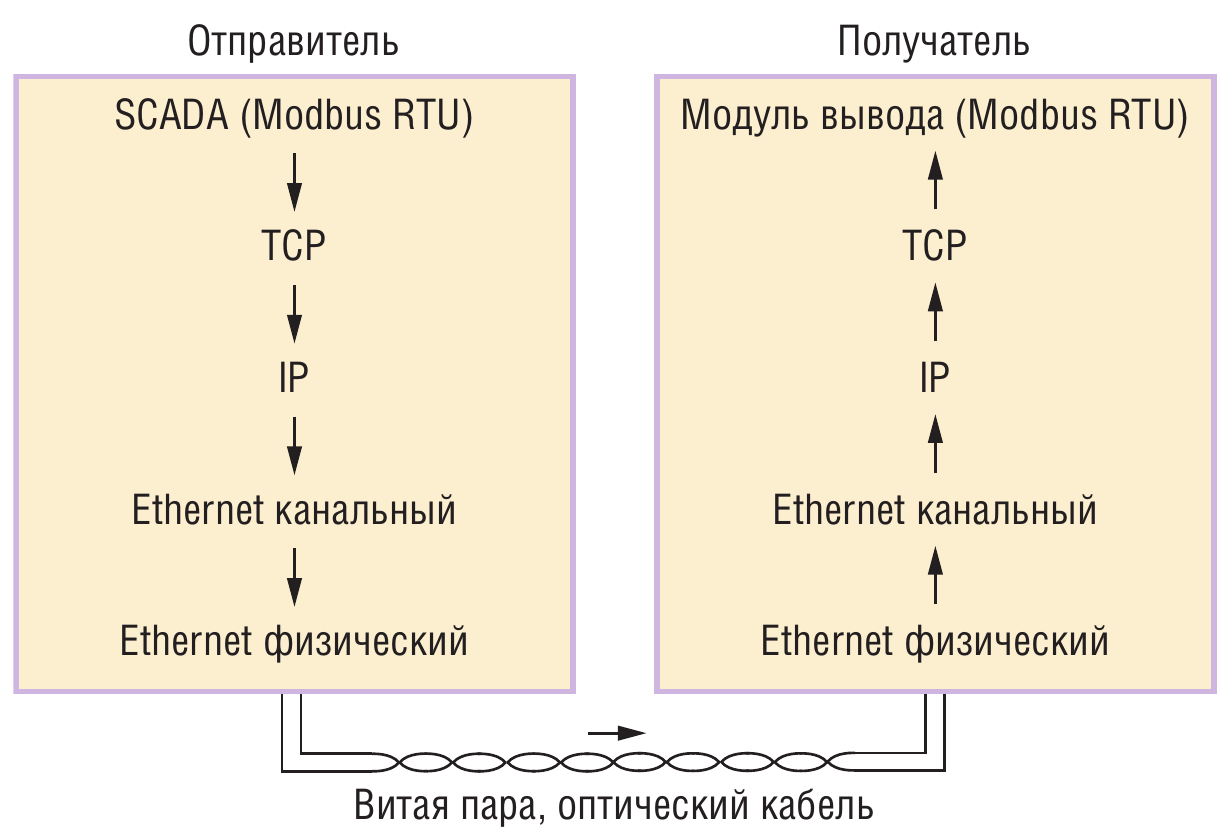
\includegraphics[width=0.7\linewidth]{images/modbus_tcp}
	\caption{Процесс передачи пакетов \mb \textit{RTU} по сети \tcp}
	\label{fig:modbustcp_ip}
\end{figure}


Более подробно о работе с протоколом \mb{} можно узнать в документации \cite{swales_open_1999}. 